\item
In this problem, you will conduct the stability analysis of a parallel  PAA identification algorithm. The system that we want to identify is the second-order system given by
\begin{align*}
    y(k) = \frac{b_1q^{-1} + b_2 q^{-2}}{1 + a_1 q^{-1} + a_2 q^{-2}} u(k) \; .
\end{align*}
Note that the system dynamics can be written as
\begin{align*}
    y(k+1) & = \theta^T \phi(k) \\
    \phi(k) & = \begin{bmatrix}
            -y(k) & -y(k-1) & u(k) & u(k-1)
        \end{bmatrix}^T \\
    \theta & = \begin{bmatrix}
            a_1 & a_2 & b_1 & b_2
        \end{bmatrix}^T \; .
\end{align*}
The PAA uses a parallel model and is governed by the equations
\begin{align}
    \hat{\phi}(k) & = \begin{bmatrix}
            -\hat{y}(k) & -\hat{y}(k-1) & u(k) & u(k-1)
        \end{bmatrix}^T
        \label{eq:parallel_PAA_first} \\
    \hat{y}^o(k+1) & = \hat{\theta}^T(k) \, \hat{\phi}(k) \\
    e^o(k+1) & =  y(k+1) - \hat{y}^o(k+1) \\
    v^o(k+1) & = e^o(k+1) + c_1 \, e(k) + c_2 \, e(k-1) \\
    v(k+1) & = \frac{ \lambda_1(k) }{ \lambda_1(k) + \hat{\phi}^T(k) F(k) \hat{\phi}(k) } v^o(k+1) \\    \hat{\theta}(k+1) & = \hat{\theta}(k) + \frac{1}{\lambda_1(k)} F(k) \hat{\phi}(k)\,v(k+1) \\
    \hat{y} (k+1) & = \hat{\theta}^T(k+1) \hat{\phi}(k) \\
    e(k+1) & = y(k+1) - \hat{y}(k+1) \\
    F(k+1) & = \frac{1}{\lambda_1(k)} \, \left[ F(k) - \lambda_2(k)
        \frac{ F(k) \hat{\phi}(k) \hat{\phi}^T(k)F(k) }
        { \lambda_1(k) + \lambda_2(k) \hat{\phi}^T(k)F(k) \hat{\phi}(k) } \right]
        \label{eq:parallel_PAA_last}
\end{align}
where $0 < \lambda_1(k) \leq 1$, $0 \leq \lambda_2(k) < 2$ and the constants $c_1$ and $c_2$ must be selected so that the transfer function
\begin{align}
    \label{eq:gq}
    G(z^{-1}) = \frac{1 + c_1 \, z^{-1} + c_2\, z^{-2}}{ 1 + a_1 \, z^{-1} + a_2\, z^{-2}}
\end{align}
has the necessary properties. (You will determine what these properties are.)

\begin{enumerate}
    \item
    Show that $v(k+1) = e(k+1) + c_1 e(k) + c_2 e(k-1)$.

    \item
    Using the result of the previous part, show that the relationship
    \begin{equation}
    \begin{aligned}
        v(k) & = G(q^{-1}) m(k) \\
        m(k) & = \tilde{\theta}^T(k) \hat{\phi}(k-1)
    \end{aligned} \label{eq:efl}
    \end{equation}
    holds, where $G(z^{-1})$ is given by Eq. \eqref{eq:gq}, and $\tilde{\theta}(k) = \theta - \hat{\theta}(k)$.

    \textbf{Hint:} As the first step in the proof, use the expressions for $y(k+1)$ and $\hat{y}(k+1)$ to show that
    \begin{align}
        e(k+1) = - a_1 e(k) - a_2 e(k - 1) + m(k+1) \; .
        \label{eq:ek_mk}
    \end{align}
    Then use the result of part (a) to complete the problem.

    \item
    Using the results of the previous part, the PAA error dynamics can be represented by the block diagram in Fig.~\ref{fig:hyperstability_basic_block}.
    \begin{figure}[h]
        \centering
        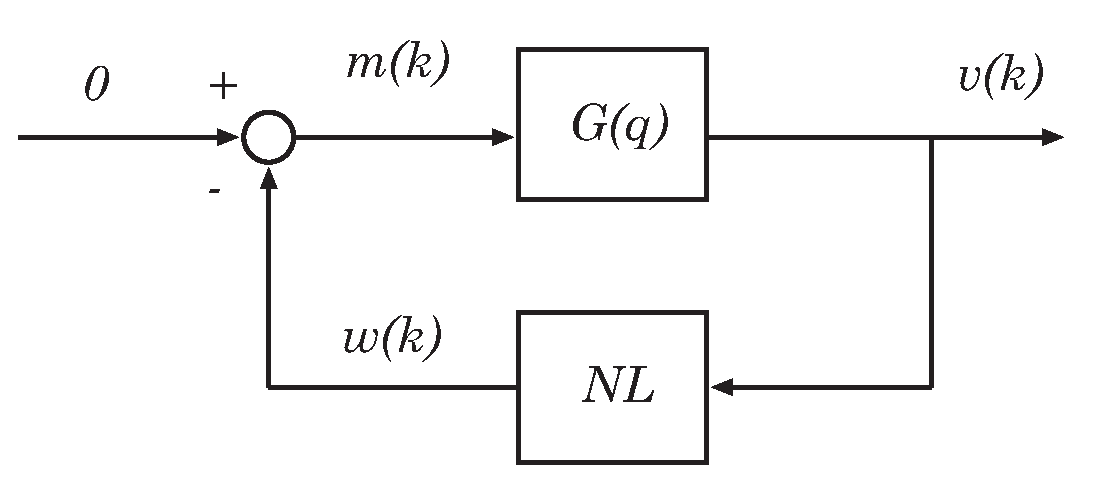
\includegraphics[width=6cm]{hyperstability_basic_block}
        \caption{Parallel PAA error dynamics}
        \label{fig:hyperstability_basic_block}
    \end{figure}
    Perform the same series of block diagram operations to the block diagram in Fig.~\ref{fig:hyperstability_basic_block} as were performed in Lecture 21 on slides 26--31. The resulting equivalent feedback loop should have an LTI system in negative feedback with a \underline{P-class} nonlinear block.

    \item
    State the properties that $G(z^{-1})$ must satisfy in order to use the asymptotic hyperstability theorem to prove asymptotic hyperstability of the equivalent feedback loop determined in part (c).

    \item
    Under the conditions determined in the previous part, show that $e^o(k)$, $e(k)$, $v^o(k)$, and $v(k)$ converge to zero. Assume that $u(k)$ and $F(k)$ are bounded.
\end{enumerate} 